\subsection{Audio}
\label{subsec:intro-audio}

\begin{figure}[H]
    \centering
    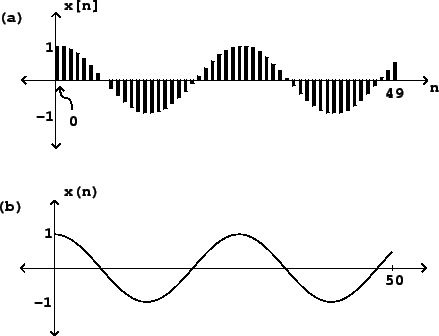
\includegraphics[scale=0.6]{imagenes/signals.png}
    \caption{Señales de audio}
    \label{fig:signals}
\end{figure}

Simplificándolo extremamente, una señal de audio (\textbf{(b)} en la figura \ref{fig:signals}) es una representación del sonido, que puede ser visualizado como una curva continua (en el caso analógico, sus valores representan voltaje eléctrico) en función del tiempo. Al digitalizar una señal, se discretiza la curva (\textbf{(a)} en la figura \ref{fig:signals}) tomando valores cada cierta cantidad de tiempo, lo que da lugar a la \textit{frecuencia de muestreo} (\textbf{sampling rate}, expresada como cantidad de muestras por segundo, unidad \textbf{Hz}). A la vez, cada uno de esos valores no puede ser expresado con precisión infinita, sino que al pasar al dominio digital, debe poder ser representado con una cantidad específica de bits, lo que origina la \textit{tasa de bits} (\textbf{bit rate}, \textit{resolución} de una señal de audio). \vspace{\baselineskip}

El formato de audio elegido para el \textbf{TP} es WAV \footnote{Más información aquí: \\ \url{http://stackoverflow.com/questions/13039846/what-do-the-bytes-in-a-wav-file-represent}}, por ser uno de los más simples para manipular. Los datos correspondientes al audio no están comprimidos, por lo que es posible realizar directamente sobre ellos las operaciones necesarias para aplicar los diversos efectos. En caso de que un archivo sea \textbf{stereo}, la información va intercalada (una muestra del canal izquierdo, otra del derecho, la siguiente del izquierdo, etc.).\vspace{\baselineskip}

La librería utilizada para el manejo de este tipo de archivo se verá en la sección \fullref{subsec:libsndfile}.\vspace{\baselineskip}

\fbox{\begin{minipage}{42em}
\underline{Nota}: por recomendación del profesor durante la presentación del proyecto de \textbf{TP}, en el archivo de audio final obtenido luego de la aplicación de alguno de los efectos, la \textit{señal seca} (\textit{dry sound/dry signal}, sin efecto) va por un canal, y la \textit{señal húmeda} (\textit{wet sound/wet signal}) por el otro. De este modo, se puede apreciar con mayor claridad el efecto en cuestión. 

\ \ \ \ Esto implica que todos los archivos de salida tendrán dos canales (\textbf{stereo}), a pesar de que el archivo de entrada pudiera haber tenido un único canal. En el caso de archivos de entrada con dos canales, se realiza un promedio de ambos (aunque esto sólo es válido en archivos stereo que mandan el mismo audio por los canales), y sobre ese nuevo ``canal'' se aplica el efecto correspondiente.
\end{minipage}} 
\label{output-stereo}